\subsection{Kinematics in Cartesian Coordinates}
\begin{frame}
\frametitle{Kinematics in Cartesian Coordinates}
The velocity and acceleration are just the \alert{Derivatives} of the \alert{position vector}.
\begin{block}{Position Vector}
\[\overline{r}(t)=x(t)\hat{n}_x+y(t)\hat{n}_y+z(t)\hat{n}_z\]
\end{block}
\begin{block}{Velocity}
\[\overline{v}(t)=\dot{\overline{r}}(t)=\dot x(t)\hat{n}_x+\dot y(t)\hat{n}_y+\dot z(t)\hat{n}_z\]
Instantaneous \alert{Speed} $v=\sqrt{\dot{x}^2+\dot{y}^2+\dot{z}^2}$
\end{block}
\begin{block}{Acceleration}
\[\overline{a}(t)=\dot{\overline{v}}(t)=\ddot x(t) \hat n_x+\ddot y(t)\hat n_y+\ddot z(t)\hat n_z\]
$a=\sqrt{\ddot x^2+\ddot y^2+\ddot z^2}$
\end{block}
\end{frame}
\subsection{Kinematics in Cylindrical Coordinates}
\begin{frame}
\frametitle{Derivatives of Versors w.r.t. Time}
Based on the \alert{position vector}, we find the \alert{velocity} and \alert{acceleration}.
\begin{block}{Position Vector in Cylindrical Coordinates}
\[\overline{r}(t)=\rho(t)\hat n_\rho+z(t)\hat n_z\]
\end{block}
\begin{block}{Relation Between Versors}
\[\hat n_\rho=\hat n_x\cos\varphi+\hat n_y\sin\varphi\quad \hat n_\varphi=-\hat n_x\sin\varphi+\hat n_y\cos\varphi\quad \hat n_z=\hat n_z\]
\end{block}
\begin{block}{Derivatives of Versors}
\[\dot{\hat{n}}_\rho=-\hat n_x\dot\varphi\sin\varphi+\hat n_y\dot \varphi\cos\varphi=\dot\varphi\hat n_\varphi \]
\[\dot{\hat{n}}_\varphi=-\hat n_x\dot\varphi\cos\varphi-\hat n_y\dot\varphi\sin\varphi=-\dot\varphi \hat n\rho\]
\end{block}
Then using the \alert{product rule} of differentiation, we calculate velocity and acceleration.
\end{frame}
\begin{frame}
\frametitle{Velocity and Acceleration in Cylindrical Coordinates}
\alert{$\dot{\hat{n}}_\rho=\dot\varphi\hat n_\varphi$} and \alert{$\dot{\hat{n}}_\varphi=-\dot\varphi \hat n\rho$} are used in the following derivation.
\begin{block}{Velocity}
\[\overline{v}=\dot\rho\hat n_\rho+\alert{\rho\dot{\hat{n}}_{\rho}}+\dot z\hat n_z=\dot\rho\hat n_\rho+\rho\dot\varphi\hat n_\varphi+\dot z\hat n_z\]
\end{block}
\begin{block}{Acceleration}
\begin{align*}\overline{a}&=\ddot\rho\hat n_\rho+\alert{\dot\rho\dot{\hat{n}}_\rho}+\dot\rho\dot\varphi\hat n_\varphi+\rho\ddot\varphi\hat n_\varphi+\alert{\rho\dot\varphi\dot{\hat{n}}_\varphi}+\ddot z\hat n_z\\
&=\ddot\rho\hat n_\rho+\alert{\dot\rho  \dot\varphi\hat n_\varphi}+\dot\rho\dot\varphi\hat n_\varphi+\rho\ddot\varphi\hat n_\varphi+\alert{\rho\dot\varphi   (-\dot\varphi \hat n\rho)}+\ddot z\hat n_z\\
&=\underbrace{(\ddot\rho-\rho\dot\varphi^2)\hat n_\rho}_{\text{\alert{radial} component}}+\underbrace{(\rho\ddot\varphi+2\dot\rho\dot\varphi)\hat n_\varphi}_{\text{\alert{transversal} component}}+\ddot z\hat n_z
\end{align*}
\end{block}
Setting \alert{$z\equiv 0$} in the preceding formulas yields the formulas for the \alert{polar coordinates}.
\end{frame}
\subsection{Kinematics in Spherical Coordinates}
\begin{frame}
\begin{block}{Position Vector in Spherical Coordinates}
\[\overline{r}(t)=r(t)\hat n_r\]
\end{block}
\alert{Relation Between Versors}
\begin{align*}\hat n_r&=\sin\theta(\hat n_x\cos\varphi+\hat n_y\sin\varphi)+\hat n_z\cos\theta\\
\hat n_\varphi&=-\hat n_x\sin\varphi+\hat n_y\cos\varphi\\
\hat n_\theta&=\cos\theta(\hat n_x\cos\varphi+\hat n_y\sin\varphi)
\end{align*}

\begin{block}{Derivatives of Versors w.r.t. Time}
\[\dot{\hat{n}}_r=\dot\theta\hat n_\theta+\dot\varphi\sin\theta\hat n_\varphi\]\[ \dot{\hat{n}}_\varphi=-\dot\varphi\sin\theta\hat n_r-\dot\varphi\cos\theta\hat n_\theta\]\[ \dot{\hat{n}}_\theta=-\dot\theta\hat n_r+\dot\varphi\cos\theta\hat n_\varphi\]
\end{block}
\end{frame}
\subsection{Kinematics in Natural Coordinates}
\begin{frame}
\frametitle{Natural Coordinates}
\begin{picture}(200,200)
\put(0,70){\includegraphics[width=200pt]{NaturalCoordinates.png}}
\put(200,180){Versors:}
\put(200,160){$\hat n_\tau$: tangent (along $\overline{v}$)}
\put(200,140){$\hat n_n$: normal}
\put(200,120){$\hat n_b$: binormal}
\put(200,100){Velocity:}
\put(200,80){$\overline{v}(t)=v\hat n_\tau$}
\put(200,60){$\hat n_\tau=\frac{\overline{v}}{v}=\frac{\dot{\overline{r}}}{|\dot{\overline{r}}|}$}
\put(0,45){Assumption: the trajectory is not straight;}
\put(25,30){the particle moves in one direction.}
\put(100,15){$\hat{n}_n=\frac{\dot{\hat{n}}_\tau}{|\dot{\hat{n}}_\tau|}$\quad $\hat{n}_b=\hat n_\tau\times \hat n_n$}
\end{picture}
\end{frame}
\begin{frame}
\frametitle{Acceleration and Curvature}
\begin{block}{Acceleration}
\[\overline{a}=\underbrace{\dot{v}\hat n_\tau}_{\text{\alert{tangent} component}}+\underbrace{v|\dot{\hat{n}}_{\tau}|\hat n_n}_{\text{\alert{normal} component}}\]
\end{block}
\begin{block}{Radius of Curvature}
\[R_c=\frac{v}{|\dot{\hat{n}}_\tau|}\]
\[\overline{a}=\underbrace{\dot{v}\hat n_\tau}_{\text{\alert{tangential} component }\overline{a}_\tau}+\underbrace{(v^2/R_c) \hat n_n}_{\text{\alert{normal} component }\overline{a}_n}\]
\end{block}
\end{frame}
\subsection{Discussion}
\begin{frame}
\frametitle{The Difference Between $\dot{\mathbf{v}}$ and $\dot v$}
The derivative of a \alert{vector} $\mathbf{v}$ is the \alert{vector} whose components are \alert{derivatives of the components} in the original vector. It is exactly the \alert{\textbf{acceleration}} of the particle. The derivative of a \alert{scalar} $v$ is the \alert{rate of change} of the \alert{magnitude} of velocity. It is precisely the magnitude of the \alert{\textbf{tangential component}} of acceleration.
\begin{example}
Consider a particle moving with velocity $\overline{v}(t)=\left(\begin{matrix}t\\t^2\\t^3\end{matrix}\right)$, so $\dot{\overline{v}}=\left(\begin{matrix}1\\2t\\3t^2\end{matrix}\right)$. Now $v=\sqrt{t^2+t^4+t^6}$, so $\dot v=\frac{2t+4t^3+6t^5}{2\sqrt{t^2+t^4+t^6}}$.\\
Now the \alert{unit tangent vector} $\hat n_\tau=\frac{v}{|v|}=\frac{1}{\sqrt{t^2+t^4+t^6}}\left(\begin{matrix}t\\t^2\\t^3\end{matrix}\right)$
\end{example}
\end{frame}
\begin{frame}
\begin{example}
\frametitle{$\dot v$ as Magnitude of Tangential Component of $\mathbf{a}$}
Now the \alert{tangential} component and \alert{normal} component of the acceleration can be calculated using the \alert{inner product} of these unit vectors and \alert{acceleration}. The \alert{magnitude} $a_\tau=\left<\overline{a},\hat n_\tau\right>$ and $a_n=\left<\overline{a},\hat n_n\right>$.
\[a_\tau=\frac{1}{\sqrt{t^2+t^4+t^6}}\left<\left(\begin{matrix}1\\2t\\3t^2\end{matrix}\right),\left(\begin{matrix}t\\t^2\\t^3\end{matrix}\right)\right>=\frac{t+2t^3+3t^5}{\sqrt{t^2+t^4+t^6}}\alert{=\dot v}\]
This results conforms with the assertion that \alert{$\dot v$} is just the \alert{magnitude} of the \alert{tangential component $\overline{a}_\tau$} of the \alert{acceleration $\overline{a}=\dot{\overline{v}}$}.
\end{example}
Then, applying the \alert{quotient rule} for the derivative, we find the \alert{unit normal vector}:
\end{frame}
\begin{frame}
\begin{example}
\frametitle{Calculating $\hat n_n$}
\[\dot{\hat{n}}_\tau=\frac{1}{t^2+t^4+t^6}\left(\begin{matrix}\sqrt{t^2+t^4+t^6}-t\frac{2t+4t^3+6t^5}{2\sqrt{t^2+t^4+t^6}}\\2t\sqrt{t^2+t^4+t^6}-t^2\frac{2t+4t^3+6t^5}{2\sqrt{t^2+t^4+t^6}}\\3t^2\sqrt{t^2+t^4+t^6}-t^3\frac{2t+4t^3+6t^5}{2\sqrt{t^2+t^4+t^6}}\end{matrix}\right)\]
\[
|\dot{\hat{n}}_\tau|=\frac{\sqrt{t^4+4t^6+t^8}}{t^2+t^4+t^6}
\]
\[\hat n_n=\frac{\dot{\hat{n}}_\tau}{|\dot{\hat{n}}_\tau|}=\frac{1}{\sqrt{t^4+4t^6+t^8}}\left(\begin{matrix}\sqrt{t^2+t^4+t^6}-t\frac{2t+4t^3+6t^5}{2\sqrt{t^2+t^4+t^6}}\\2t\sqrt{t^2+t^4+t^6}-t^2\frac{2t+4t^3+6t^5}{2\sqrt{t^2+t^4+t^6}}\\3t^2\sqrt{t^2+t^4+t^6}-t^3\frac{2t+4t^3+6t^5}{2\sqrt{t^2+t^4+t^6}}\end{matrix}\right)
\]
\end{example}
\end{frame}
\begin{frame}
\frametitle{Calculating $a_n$}
\begin{example}
\begin{align*}
a_n&=\frac{1}{\sqrt{t^4+4t^6+t^8}}\left<\left(\begin{matrix}1\\2t\\3t^2\end{matrix}\right),\left(\begin{matrix}\sqrt{t^2+t^4+t^6}-t\frac{2t+4t^3+6t^5}{2\sqrt{t^2+t^4+t^6}}\\2t\sqrt{t^2+t^4+t^6}-t^2\frac{2t+4t^3+6t^5}{2\sqrt{t^2+t^4+t^6}}\\3t^2\sqrt{t^2+t^4+t^6}-t^3\frac{2t+4t^3+6t^5}{2\sqrt{t^2+t^4+t^6}}\end{matrix}\right)\right>\\
&=\frac{\sqrt{t^8+4 t^6+t^4}}{\sqrt{t^6+t^4+t^2}}
\end{align*}
and we can check that \alert{$a_n^2+a_\tau^2=a^2$}
\end{example}

\end{frame}
\begin{frame}
\frametitle{Role of the normal component $\mathbf{a}_n$}
\begin{block}{Remarks}
\[
\hat n_\tau\circ\hat n_\tau=1\implies \frac{\derivative}{\derivative t}[\hat n_\tau\circ\hat n_\tau]=0\implies \frac{\derivative}{\derivative t}\hat n_\tau \circ \hat n_\tau+\hat n_\tau\circ\frac{\derivative}{\derivative t}\hat n_\tau=0
\]
Notice that $\dot{\hat{n}}_\tau$ is \alert{perpendicular} to $\hat n_\tau$ because $\hat n_\tau$ has \alert{unit length}.
The \alert{normal component} of acceleration, therefore, only changes the \alert{direction} of velocity, and has no effect on the magnitude of velocity.
\end{block}
\end{frame}
\begin{frame}
\frametitle{Differential Geometry in Polar Coordinates}
Changing $r$ ,keeping $\varphi$ constant, results in displacement \alert{along} $\overline{r}$, while changing $\varphi$, keeping $r$ constant, results in displacement \alert{perpendicular} to $\overline{r}$. Putting these two kinds of changes in the form of \alert{infinitesimal displacement vector}: $\hat n_r \derivative r$ and $\hat n_\varphi r\derivative \varphi$, we note that in fact, \[
\underbrace{\derivative \overline{r}}_{\text{\alert{Infinitesimal displacement}}}=\underbrace{\hat n_r \derivative r}_{\text{\alert{Radial} Component}}+\underbrace{\hat n_\varphi r\derivative\varphi}_{\text{\alert{Transversal} Component}}
\]
Therefore, by the \alert{Pythagoras' theorem},
\[
|\derivative \overline{r}|^2=(\derivative r)^2+(r\derivative\varphi)^2
\]
In fact, this is exactly the case for \alert{velocity}: we can decompose the velocity into \alert{radial} and \alert{transversal} components, and exploit the fact that they are \alert{mutually perpendicular} to each other.
\end{frame}
\subsection{Exercises}
\begin{frame}
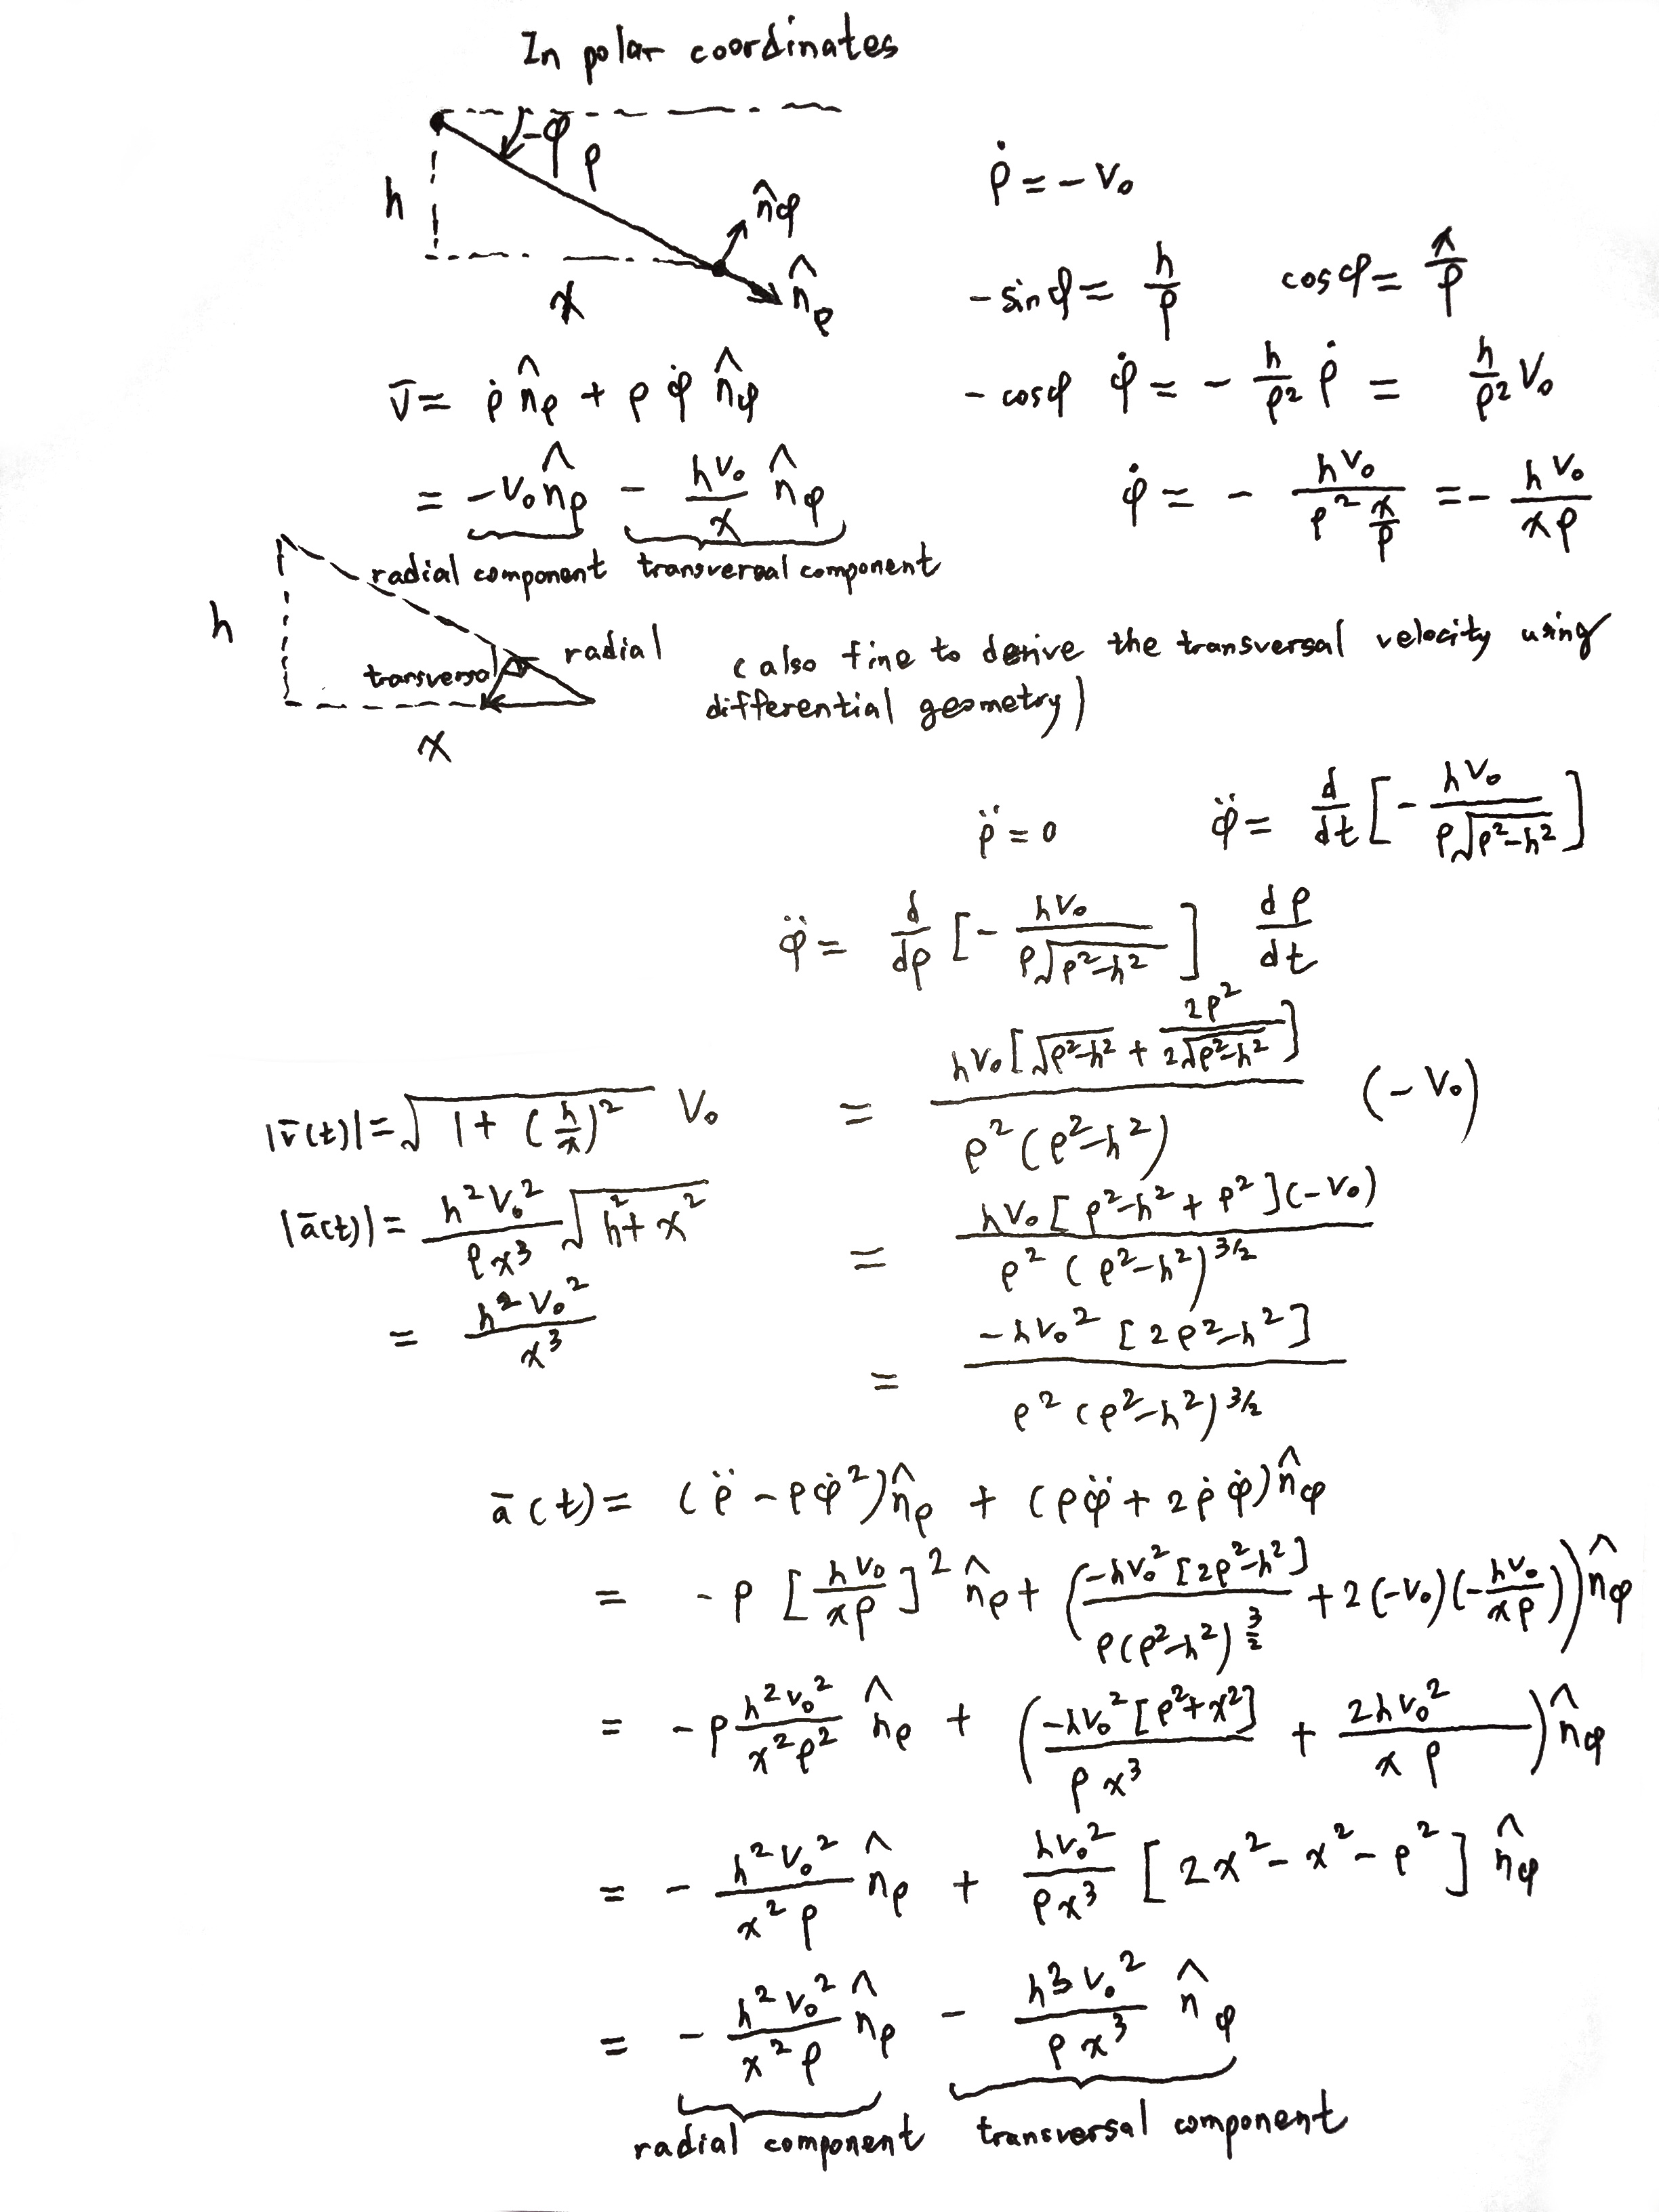
\includegraphics[height=8cm]{RC2PullingBoatRevisited.JPG}
\end{frame}
\begin{frame}
\begin{block}{A Parabolic Motion}
A particle moves in the $x-y$ plane so that
\[x(t)=at,\quad y(t)=bt^2\]
where $a,b$ are positive constants. Find its trajectory, velocity, and acceleration (its tangential and normal components).
\end{block}
\begin{block}{Solution}
The \alert{trajectory} is $y=b(x/a)^2$. The \alert{position vector} $\overline{r}=\left(\begin{matrix}at\\bt^2\end{matrix}\right)$, so the \alert{velocity} is $\dot{\overline{r}}=\left(\begin{matrix}a\\2bt\end{matrix}\right)$. The \alert{acceleration} is $\ddot{\overline{r}}=\left(\begin{matrix}0\\2b\end{matrix}\right)$.\\The \alert{unit tangent vector} $\hat n_\tau=\frac{\overline{v}}{v}=\frac{1}{\sqrt{a^2+4b^2t^2}}\left(\begin{matrix}a\\2bt\end{matrix}\right)$.
\end{block}
\end{frame}
\begin{frame}
\frametitle{A Parabolic Motion}
\begin{block}{Solution (Continued)}
The \alert{tangential} component of acceleration $\mathbf{a}_\tau=\left<\overline{a},\hat n_\tau\right>\hat n_\tau$ \[\mathbf{a}_\tau=\frac{4b^2t}{\sqrt{a^2+4b^2t^2}}\frac{1}{\sqrt{a^2+4b^2t^2}}\left(\begin{matrix}a\\2bt\end{matrix}\right)=\frac{1}{a^2+4b^2t^2}\left(\begin{matrix}4ab^2t\\8b^3t^2\end{matrix}\right)\]
The \alert{normal} component of acceleration $\mathbf{a}_n=\mathbf{a}-\mathbf{a}_\tau$
\[
\mathbf{a}_n=\frac{1}{a^2+4b^2t^2}\left(\begin{matrix}-4ab^2t\\2b(a^2+4b^2t^2)-8b^3t^2\end{matrix}\right)=\frac{1}{a^2+4b^2t^2}\left(\begin{matrix}-4ab^2t\\2ba^2\end{matrix}\right)
\]
\end{block}
\end{frame}
\begin{frame}
\frametitle{Relative Motion of Two Particles}
\begin{block}{Question}
The \alert{velocities} of two particles observe from a \alert{fixed frame of reference} are given in the Cartesian coordinates by vectors $\mathbf{v}_1(t)=(0,2,0)+(3,1,2)t^2$ and $\mathbf{v}_2(t)=(1,0,1)$. At the \alert{initial} instant of time $t=0$, the positions of these particles are $\mathbf{r}_1(0)=(1,0,0)$, and $\mathbf{r}_2(0)=(0,1,1)$.\\
Find the \alert{positions} of both particles and the \alert{acceleration} of particle 1 (and its tangential and normal components), \alert{relative position}, and \alert{relative acceleration} of particle 1 with respect to particle 2 at any instant of time 
$t$.
\end{block}
\end{frame}
\begin{frame}
\frametitle{Relative Motion of Two Particles (Solution)}
The \alert{positions} are found as follows:\\
$\mathbf{r}_1(t)=\mathbf{r}_1(0)+\int_0^t\mathbf{v}_1(\tau)\derivative\tau=(1,0,0)+(0,2,0)t+(1,1/3,2/3)t^3$\\
$\mathbf{r}_2(t)=\mathbf{r}_2(0)+\int_0^t\mathbf{v}_2(\tau)\derivative\tau=(0,1,1)+(1,0,1)t$\\
The \alert{acceleration} of particle 1 and 2 are found as follows:\\
$\mathbf{a}_1(t)=\dot{\mathbf{v}}_1(t)=(6,2,4)t$ \quad $\mathbf{a}_2(t)=\overline{0}$\\
The \alert{unit tangent vector} for particle 1 is found as $\hat{n}_{\tau,1}=\frac{\mathbf{v}_1(t)}{|\mathbf{v}_1(t)|}=\frac{1}{\sqrt{9t^4+(2+t^2)^2+4t^4}}[(0,2,0)+(3,1,2)t^2]$
\\
so the \alert{tangential component} of acceleration is found as
$\mathbf{a}_{\tau,1}=\left<\mathbf{a}_1(t),\hat{n}_{\tau,1}\right>\hat{n}_{\tau,1}=\frac{t(18t^2+4+2t^2+8t^2)}{9t^4+(2+t^2)^2+4t^4}[(0,2,0)+(3,1,2)t^2]$
\end{frame}
\begin{frame}
\frametitle{Relative Motion of Two Particles (Continued Solution)}
$\mathbf{a}_{\tau,1}=\frac{2 \left(7 t^3+t\right)}{7 t^4+2 t^2+2}\left(\begin{matrix}3t^2\\2+t^2\\2t^2\end{matrix}\right)$, so the \alert{normal component of accelration} $\mathbf{a}_{n,1}=\mathbf{a}_1-\mathbf{a}_{\tau,1}=\frac{1}{2+2t^2+7t^4}\left(\begin{matrix}6t(2+t^2)\\-26t^3\\4t(2+t^2)\end{matrix}\right)$. Check they are orthogornal!
The \alert{relative position} of particle 1 w.r.t. particle 2 is
\[
\mathbf{r}_1(t)-\mathbf{r}_2(t)=(1,-1,-1)+(-1,2,-1)t+(1,1/3,2/3)t^3
\]
The \alert{relative acceleration} of particle 1 w.r.t. particle 2 is
\[
\mathbf{a}_1(t)-\mathbf{a}_2(t)=(6,2,4)t
\]
\end{frame}
\begin{frame}
\frametitle{Beetle on the Wheel}
A disc of radius $R$ rotates about its axis of symmetry (perpendicular to the disk surface) with \alert{constant angular velocity} $\dot\varphi=\omega=const$. At the instant of time $t=0$ a beetle starts to walk with \alert{constant speed} $v_0$ \alert{along a radius} of the disk, from its center to the edge. Find
\begin{enumerate}
\item{the \alert{position} of the beetle and its \alert{trajectory} in the Cartesian and polar coordinate systems,}
\item{its \alert{velocity} in both systems,}
\item{its \alert{acceleration} in both systems (Cartesian components, polar components, as well as tangential and normal components).}
\end{enumerate}
\end{frame}
\begin{frame}
\frametitle{Beetle on the Wheel (Solution)}
\begin{block}{Position and Trajectory}
In the \alert{Polar} Coordinate system, $r=v_0 t$, $\varphi=\omega t$. Hence in the \alert{Cartesian} Coordinate system, $x(t)=v_0 t\cos\omega t$, $y(t)=v_0 t\sin\omega t$. The \alert{trajectory} in the Polar coordinates is $r=v_0\varphi/\omega$. The \alert{trajectory} in the Cartesian coordinates is found by \[\begin{cases}\tan\omega t&=y/x\\x^2+y^2&=v_0^2 t^2\end{cases}\]
so the trajectory is $y/x=\tan(\omega\sqrt{x^2+y^2}/v_0)$, known as \alert{Archimedes' spiral.}
\end{block}
\end{frame}
\begin{frame}
\begin{block}{Velocity}
In the \alert{Polar} Coordinate system, $\dot r=v_0$, $\dot\varphi=\omega $. Therefore, \[v_{r}=\dot r=v_0,\text{ and }v_\varphi=r\dot\varphi=v_0\omega t.\]In the \alert{Cartesian} Coordinate system, $v_x=\dot x(t)=v_0 \cos\omega t-\omega v_0 t\sin\omega t$, $v_y=\dot y(t)=v_0 \sin\omega t+\omega v_0 t\cos\omega t$.
\end{block}
\begin{block}{Acceleration}
In the \alert{Polar} Coordinate system, $\ddot r=0$, and $\ddot \varphi=0$. Therefore,
\[
a_r=\ddot r-r\dot\varphi^2=-v_0t\omega^2\text{ and }a_\varphi=r\ddot\varphi+2\dot r\dot\varphi=2v_0\omega.
\]
In the \alert{Cartesian} Coordinate system, $a_x=\ddot x(t)=-\omega v_0(2\sin\omega t+\omega t\cos\omega t)$, and $a_y=\ddot y(t)=\omega v_0(2\cos\omega t-\omega t\sin\omega t)$.
\end{block}
\textbf{CAUTION:} \alert{Tangential} component is not \alert{radial} component in this case.
\end{frame}
\begin{frame}
\frametitle{Tangential Component and Normal Component}
Based on the previous results, we calculate $v$, with which we find the \alert{magnitude} of the tangential component of acceleration.
\[v=\sqrt{v_r^2+v_\varphi^2}=v_0\sqrt{1+(\omega t)^2}\]
\[
a_\tau=\dot v=v_0\frac{\omega^2 t}{\sqrt{1+(\omega t)^2}}
\]Then we exploit the fact that the tangential and the normal components are \alert{perpendicular} to each other to find the \alert{magnitude} of the normal component from $a$:\quad
$a=\sqrt{a_r^2+a_\varphi^2}=v_0 \omega\sqrt{(\omega t)^2+4}$
\[
a_n=\sqrt{a^2-a_\tau^2}=\frac{v_0 \omega (2+(\omega t)^2)}{\sqrt{1+(\omega t)^2 }}
\]
\end{frame}
\begin{frame}
\frametitle{More on the Beetle}
\begin{enumerate}
\item{What is the \alert{distance} covered by the beetle?\begin{align*}s&=\int_0^T v\derivative t=\int_0^T v_0\sqrt{1+(\omega t)^2}\derivative t\\&=v_0 \left(\frac{1}{2} T \sqrt{\omega^2 T^2+1}+\frac{\sinh ^{-1}(\omega T)}{2 \omega}\right)\end{align*}}
\item{What is the \alert{radius of curvature} of the trajectory?\[R_c=\frac{v^2}{a_n}=\frac{v_0(1+\omega^2 t^2)^{3/2}}{\omega(2+\omega^2 t^2)}\]}
\end{enumerate}
\end{frame}
\begin{frame}
\frametitle{Hyperbolic Spiral Motion}
\begin{block}{Question}
A particle moves along a \alert{hyperbolic spiral} (i.e. a curve $r=c/\varphi$, where $c$ is a positive constant), so that $\varphi (t)=\varphi_0+\omega t$, where $\varphi_0$ and $\omega$ are positive constants. Fint its \alert{velocity} and \alert{acceleration} (all components and magnitudes of both vectors).
\end{block}
\begin{block}{Solution}
$\dot\varphi=\omega$\quad$\dot r=-c/\varphi^2\cdot\omega$, so $v_r=-c\omega/(\varphi_0+\omega t)^2$, and $v_\varphi=\omega c/(\varphi_0+\omega t)$\\$v=\sqrt{v_r^2+v_\tau^2}=[\omega c/(\varphi_0+\omega t)^2]\sqrt{1+(\varphi_0+\omega t)^2}$\\
$\ddot\varphi=0$\quad$\ddot r=(2\omega^2 c)/\varphi^3$, so $a_\varphi=r\ddot\varphi+2\dot r\dot \varphi=-2c\omega^2/(\varphi_0+\omega t)^2$\\
$a_r=\ddot r-r\dot{\varphi}^{2}=(2\omega^2 c)/(\varphi_0+\omega t)^3-\omega^2 c/(\varphi_0+\omega t)$\\
$a=\sqrt{a_\varphi^2+a_r^2}=\sqrt{\frac{c^2\omega^4(4+(\varphi_0+\omega t)^4)}{(\varphi_0+\omega t)^6}}$
\end{block}
\end{frame}
\begin{frame}
\frametitle{Four Crawling Spiders}
\alert{Four} spiders are initially placed at the four corners of a \alert{square} with side length $l$. The spiders crawl counter-clockwise at the \alert{same speed} $v$ and each spider crawls \alert{directly} toward the next spider at all times. They approach the center of the square along spiral paths. Find
\begin{enumerate}
\item{\alert{polar coordinates} of a spider at any instant of time, assuming the origin is at the center of the square.}
\item{the \alert{time} after which all spiders meet.}
\item{the \alert{trajectory} of a spider in polar coordinates.}
\item{the \alert{acceleration} of a spider, and the \alert{radius of curvature} at any instant of time.}
\end{enumerate}
\textbf{CAUTION:} The \alert{transversal} component is not the \alert{tangential} component in this case.
\end{frame}
\begin{frame}
\frametitle{Four Crawling Spiders (Solution)}
Due to the \alert{symmetry} of the problem, we study the spider starting at $r(0)=l/\sqrt{2}$ and $\varphi(0)=0$. \alert{Notice} that the four spiders always lie on the four corners of a square due to \alert{symmetry}. Now the fact that one spider always aims \alert{directly} at the next spider is interpreted as each spider having a \alert{radial} velocity $v_r=-v/\sqrt{2}$ and a \alert{transversal} velocity $v_\varphi=v/\sqrt{2}$. Therefore, $\dot r=-v/\sqrt{2}$ and $\dot\varphi=(v/\sqrt{2})/r(t)$. Now $r(t)=r(0)+\int_0^t \dot r(\tau)\derivative\tau=l/\sqrt{2}-vt/\sqrt{2}$, and $\varphi(t)=\varphi(0)+\int_0^t\dot\varphi(\tau)\derivative\tau$.
\[\varphi(t)=\int_0^t\frac{v}{(l-v\tau)}\derivative\tau=\int_0^{\alert{vt}}\frac{\derivative \alert{s}}{l-\alert{s}}=-\int_0^{vt}\frac{\derivative s}{s-l}=-\int_{\alert{-l}}^{\alert{vt-l}}\frac{\derivative \alert{w}}{\alert{w}}\]
so the \alert{polar coordinates} are given by \[r(t)=\frac{l-vt}{\sqrt{2}}\quad \varphi(t)=-\ln\left(\frac{vt-l}{-l}\right)\]
\end{frame}
\begin{frame}
The \alert{time} $t_f$ the spiders meet is the time when $r(t_f)=0$, so $t_f=l/v$\\The \alert{trajectory} of the spider is given by
\[
\varphi=-\ln\left(\frac{\sqrt{2}r}{l}\right)
\]
The \alert{acceleration} of the spider is given by $\mathbf{a}(t)=(\ddot{r}-r\dot\varphi^2)\hat{n}_r+(r\ddot \varphi+2\dot r\dot\varphi)\hat n_\varphi$, where $\ddot r=0$ and $\ddot\varphi=-[(v/\sqrt{2})/r(t)^2] (-v/\sqrt{2})=v^2/(l-vt)^2$. Hence,\\
$a_r=-v^2/[\sqrt{2}(l-vt)]$, \quad $a_\varphi=v^2/[\sqrt{2}(l-vt)]+\sqrt{2}(-v)(v/\sqrt{2})/[(l-vt)/\sqrt{2}]=-(\sqrt{2}-1/\sqrt{2})v^2/(l-vt)$\\
$a=\sqrt{a_r^2+a_\varphi^2}=v^2/(l-vt)$\\
Since there is no \alert{tangential} acceleration, this is the normal acceleration, so the \alert{radius of curvature} is $(l-vt)$.
\end{frame}
\begin{frame}
\frametitle{A Numerical Animation}
\animategraphics[height=2.5in,autoplay]{3}{CrawlingSpiders_}{0}{27}\\
The animation works with Adobe Reader XI or Adobe Acrobat Reader DC. Equivalent GIF is uploaded to Sakai.
\end{frame}
\begin{frame}
\lstinputlisting[breaklines=TRUE,basicstyle=\footnotesize\ttfamily,language=c++,numbers=left, numberstyle=\tiny,keywordstyle=\color{blue!40!black},commentstyle=\color{red!50!green!50!blue!50},frame=shadowbox, rulesepcolor=\color{red!20!green!20!blue!20},stringstyle=\color{orange}]{SpiderChase.cpp}
\end{frame}
